% \documentclass{article}
\documentclass[../../outputs/main.tex]{subfiles}

% Any packages or configurations specific to this section
\usepackage{lipsum}
\usepackage{graphicx}

\begin{document}

\subsection{Simulation Results}
% Case 1: centralized OPF with battery
% Case 2: ENApp based distributed OPF with battery

The Test System 

\subsubsection{Comparison between MPCOPF and MPDOPF}
In this section, comparative analyses are carried out between MPCOPF and MPDOPF considering 5-hour time steps.


% \begin{table}[h!]
%     \centering
%     \caption{Comparative analyses between MPCOPF and MPDOPF}
%     \begin{tabular}{|l|c|c|}
%     \hline
%     \textbf{Metric} & \textbf{MPCOPF} & \textbf{MPDOPF} \\ \hline
%     Line loss (kW) &   &  \\ \hline
%     Substation real power (kW) &    &   \\ \hline
%     Substation reactive power (kVAR) &    &   \\ \hline
%     PV real power (kW) &    &    \\ \hline
%     PV reactive power (kVAR) &    &   \\ \hline
%     Substation power cost (\$) &     &   \\ \hline
%     \end{tabular}
%     \label{table:combined_results_slim}
% \end{table}

% \begin{table}[h!]
%     \centering
%     \caption{Comparative analyses between MPCOPF and MPDOPF - $20 \%$ PVs and $30 \%$ Batteries for a $5$-hour}
%     \begin{tabular}{|l|c|c|}
%     \hline
%     \textbf{Metric} & \textbf{MPCOPF} & \textbf{MPDOPF} \\ \hline
%     Line loss (kW) & 75.99 & --- \\ \hline
%     Substation real power (kW) & 4308.28 & --- \\ \hline
%     Substation reactive power (kVAR) & 574.18 & --- \\ \hline
%     PV reactive power (kVAR) & 116.92 & --- \\ \hline
%     Substation power cost (\$) & 576.31 & --- \\ \hline
%     Number of Iterations & 1 & --- \\ \hline
%     Total Simulation Time (s) & 521.25 & --- \\ \hline
%     \end{tabular}
%     \label{table:opt-5-20-30}
% \end{table}

% \begin{table}[h!]
%     \centering
%     \caption{Comparative analyses between MPCOPF and MPDOPF - $5$ time-period horizon}
%     \begin{tabular}{|l|c|c|}
%     \hline
%     \textbf{Metric} & \textbf{MPCOPF} & \textbf{MPDOPF} \\ \hline
%     Substation power cost (\$) & 576.31 & 576.30 \\ \hline
%     Substation real power (kW) & 4308.28 & 4308.14 \\ \hline
%     Line loss (kW) & 75.99 & 76.12 \\ \hline
%     Substation reactive power (kVAR) & 574.18 & 656.24 \\ \hline
%     PV reactive power (kVAR) & 116.92 & 160.64 \\ \hline
%     Battery reactive power (kVAR) & 202.73 & 76.01 \\ \hline
%     Number of Iterations & - & 5 \\ \hline
%     Total Simulation Time (s) & 521.25 & 49.87 \\ \hline
%     \end{tabular}
%     \label{table:opt-5-20-30}
% \end{table}

\begin{table}[h!]
    \centering
    \caption{Comparative analyses between MPCOPF and MPDOPF - $5$ time-period horizon}
    \begin{tabular}{|l|c|c|}
    \hline
    \textbf{Metric} & \textbf{MPCOPF} & \textbf{MPDOPF} \\ \hline
    Biggest subproblem size & \multicolumn{2}{c|}{} \\ \hline
    \quad Decision variables & {} & {} \\ \hline
    \quad Linear constraints & {} & {} \\ \hline
    \quad Nonlinear constraints & {} & {} \\ \hline
    Simulation results  & \multicolumn{2}{c|}{} \\ \hline
    \quad Substation power cost (\$) & 576.31 & 576.30 \\ \hline
    \quad Substation real power (kW) & 4308.28 & 4308.14 \\ \hline
    \quad Line loss (kW) & 75.99 & 76.12 \\ \hline
    \quad Substation reactive power (kVAR) & 574.18 & 656.24 \\ \hline
    \quad PV reactive power (kVAR) & 116.92 & 160.64 \\ \hline
    \quad Battery reactive power (kVAR) & 202.73 & 76.01 \\ \hline
    Computation  & \multicolumn{2}{c|}{} \\ \hline
    \quad Number of Iterations & - & 5 \\ \hline
    \quad Total Simulation Time (s) & 521.25 & 49.87 \\ \hline
    \end{tabular}
    \label{table:opt-5-20-30}
\end{table}


Further, here the 

\begin{table}[h!]
    \centering
    \caption{ACOPF feasibility analyses - $5$ time-period horizon}
    \begin{tabular}{|l|c|c|}
    \hline
    \textbf{Metric} & \textbf{MPDOPF} & \textbf{OpenDSS} \\ \hline
    Full horizon  & \multicolumn{2}{c|}{} \\ \hline
    \quad Substation real power (kW) & 4308.14 & 4308.35 \\ \hline
    \quad Line loss (kW) & 76.12 & 76.09 \\ \hline
    \quad Substation reactive power (kVAR) & 656.24 & 652.49 \\ \hline
    Max. all-time discrepancy & \multicolumn{2}{c|}{} \\ \hline
    \quad Voltage (pu) & \multicolumn{2}{c|}{0.0002} \\ \hline
    \quad Line loss (kW) & \multicolumn{2}{c|}{0.0139} \\ \hline
    \quad Substation power (kW) & \multicolumn{2}{c|}{0.3431} \\ \hline
    \end{tabular}
    \label{table:feas-5-20-30}
\end{table}

\begin{figure}[h!]
    \centering
    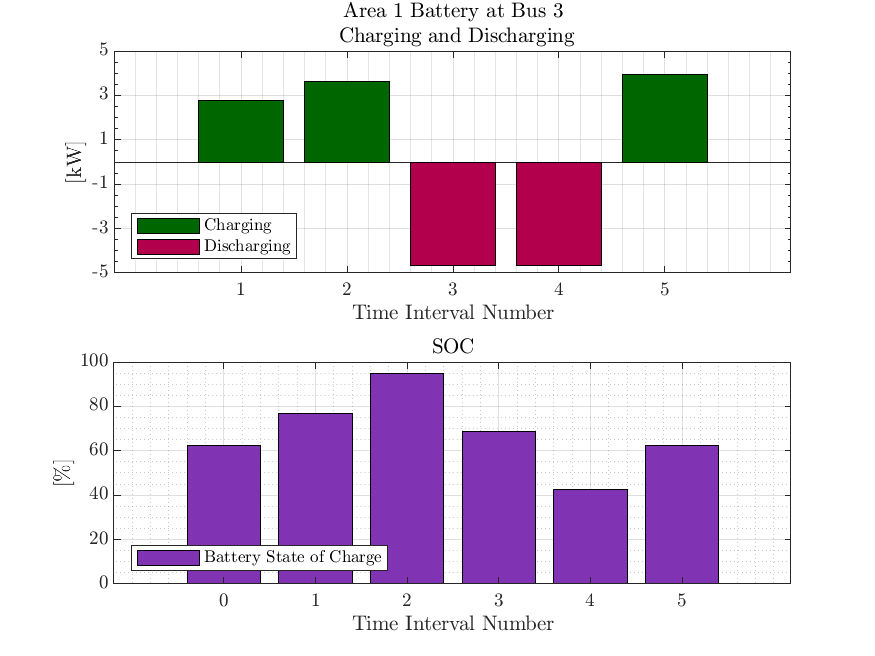
\includegraphics[width=\linewidth]{../figures/T5-pv20-batt30-genCost/dopf/BatteryPlots/macroItr_5_genCost_Battery_1_alpha_0.001.png}
    \caption{Charging-Discharging and SOC graphs for Battery at Bus 3 located in Area 1 obtained by MPDOPF}
    \label{fig:batt-plot-dopf-5-20-30-genCost}
\end{figure}

\textcolor{red}{Boundary Variable Plots are too tall, make them slightly shorter, like 25\% of the page only.}

\begin{figure*}[h!]
    \centering
    % Row 1
    \begin{subfigure}[b]{0.3\textwidth}
        \centering
        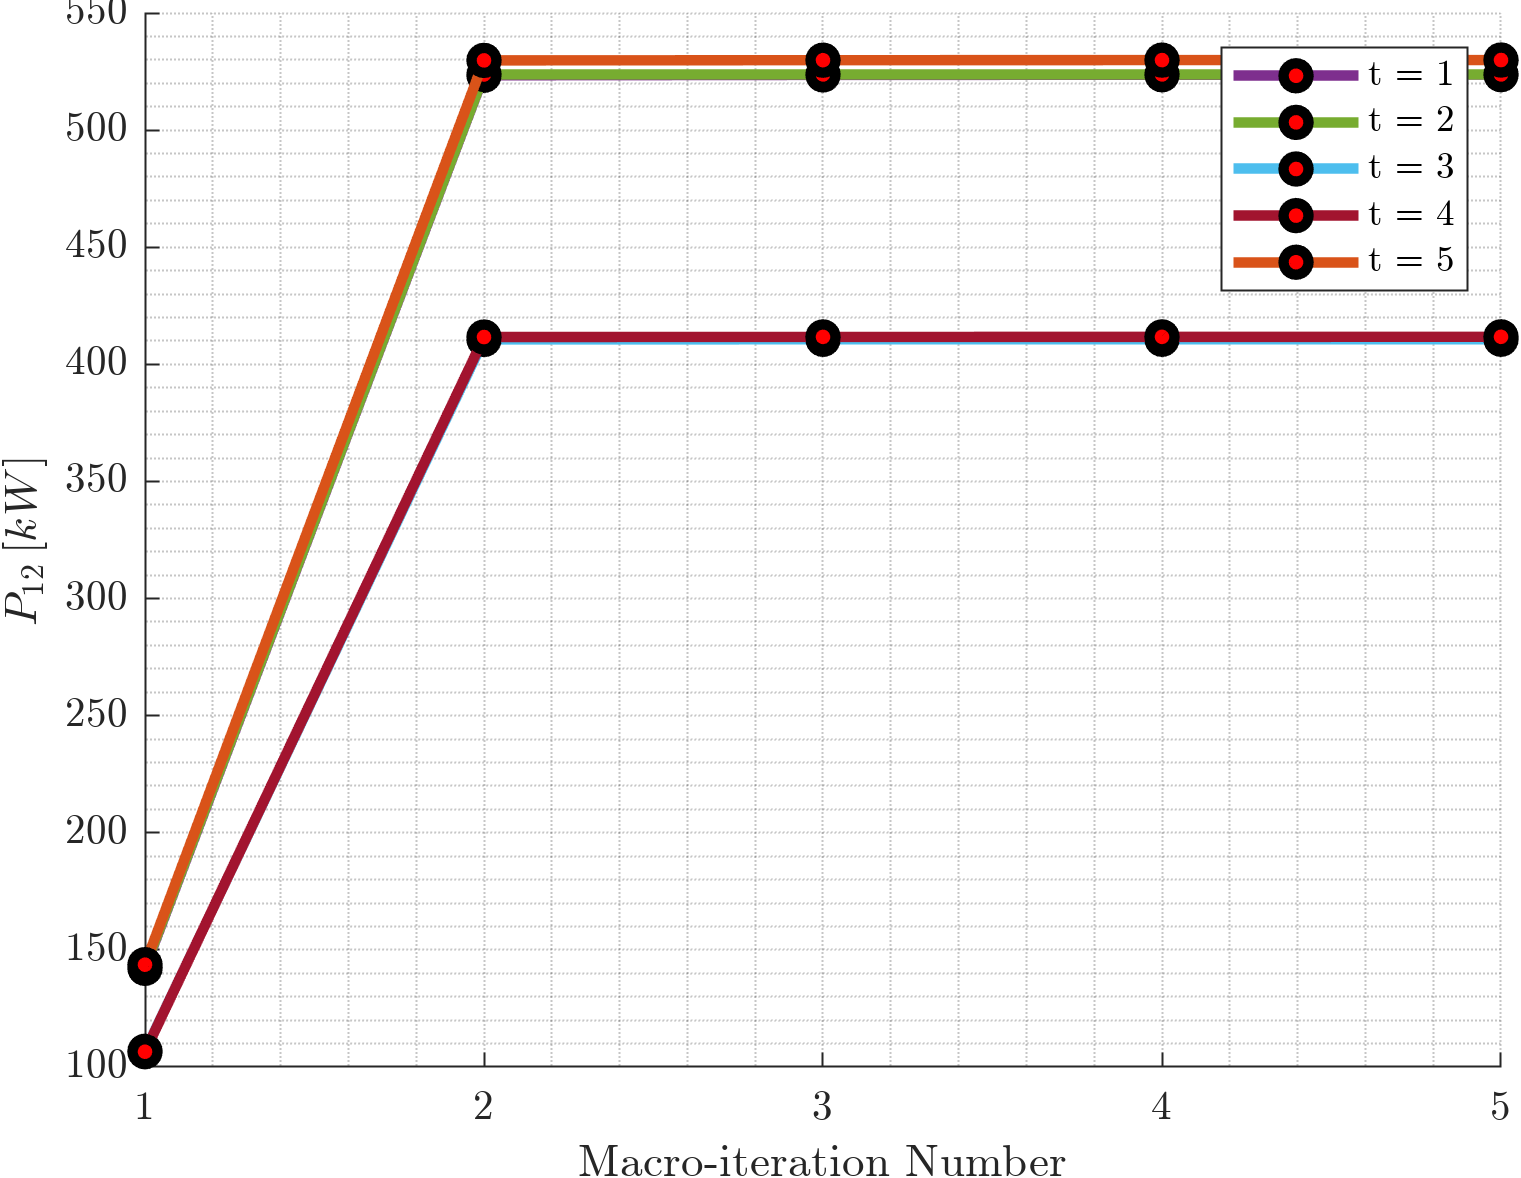
\includegraphics[width=\textwidth]{../figures/T5-pv20-batt30-genCost/dopf/convergenceCurves/BoundaryRealPower_vs_t_vs_macroItr_T_5_Areas_1_2_genCost_pv_20_batt_30_crop.png}
        \caption{\scriptsize Real Power flowing from Area $1$ into Area $2$}
        \label{fig:real_power_1_2}
    \end{subfigure}
    \hfill
    \begin{subfigure}[b]{0.3\textwidth}
        \centering
        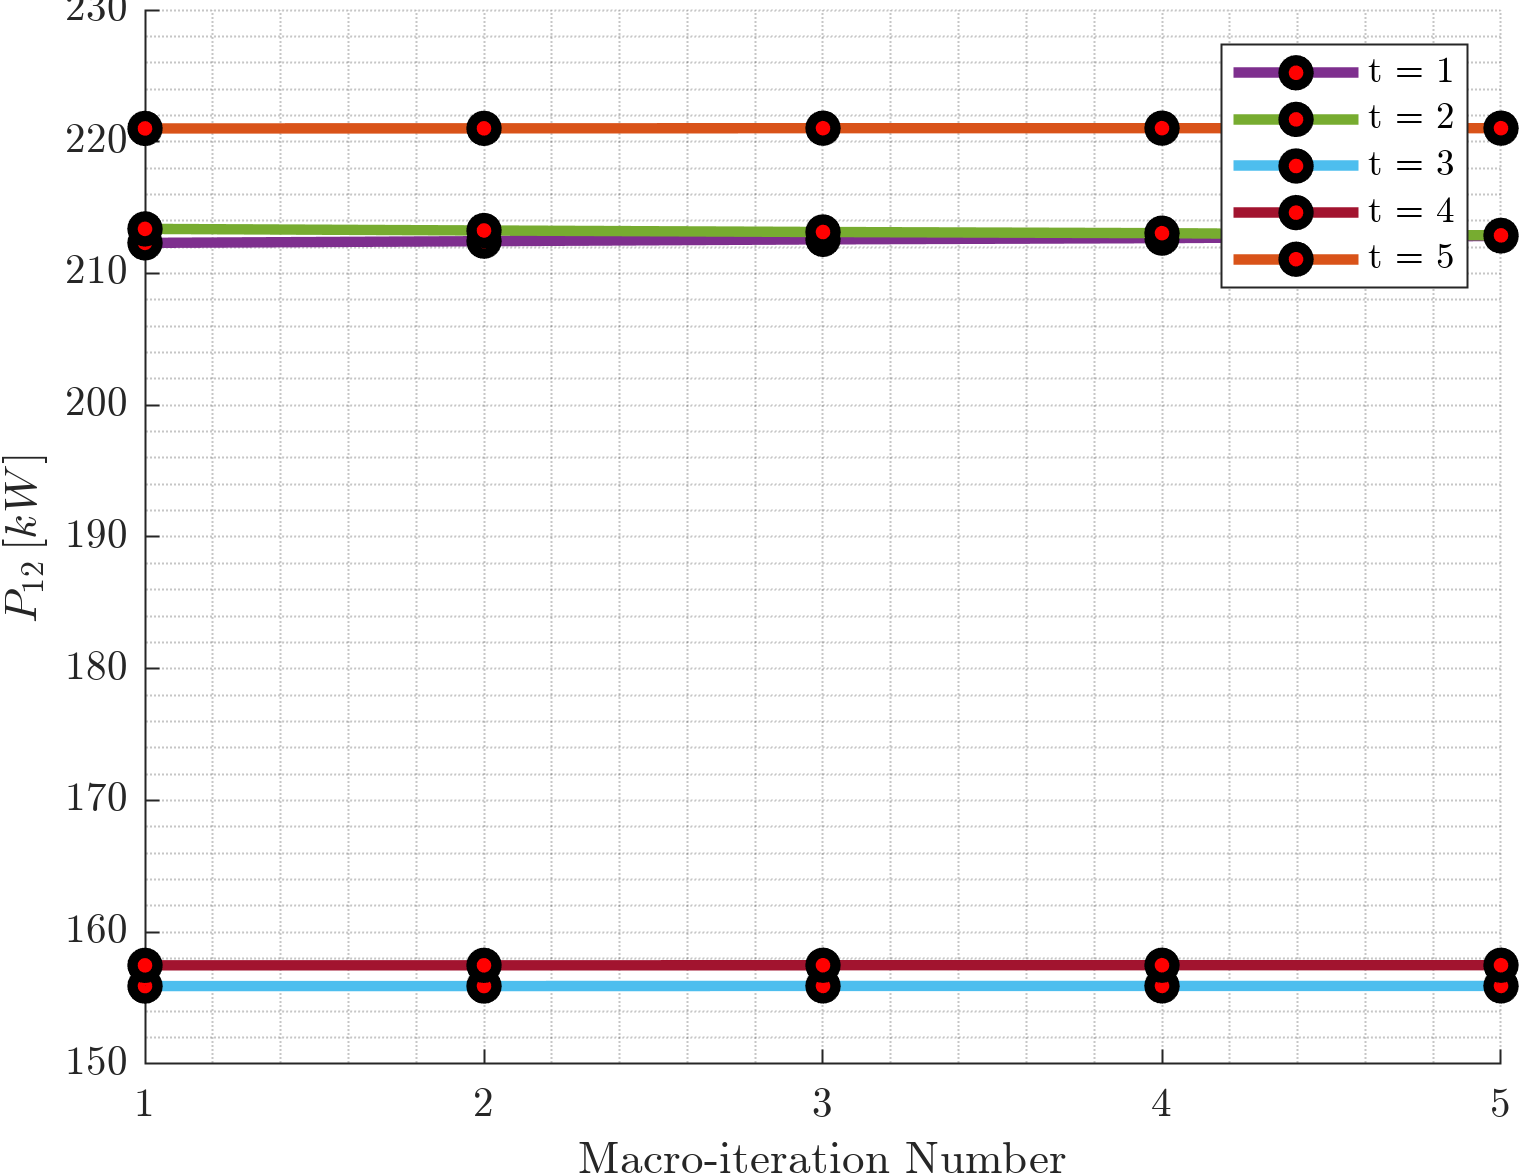
\includegraphics[width=\textwidth]{../figures/T5-pv20-batt30-genCost/dopf/convergenceCurves/BoundaryRealPower_vs_t_vs_macroItr_T_5_Areas_1_3_genCost_pv_20_batt_30_crop.png}
        \caption{\scriptsize Real Power flowing from Area $1$ into Area $3$}
        \label{fig:real_power_1_3}
    \end{subfigure}
    \hfill
    \begin{subfigure}[b]{0.3\textwidth}
        \centering
        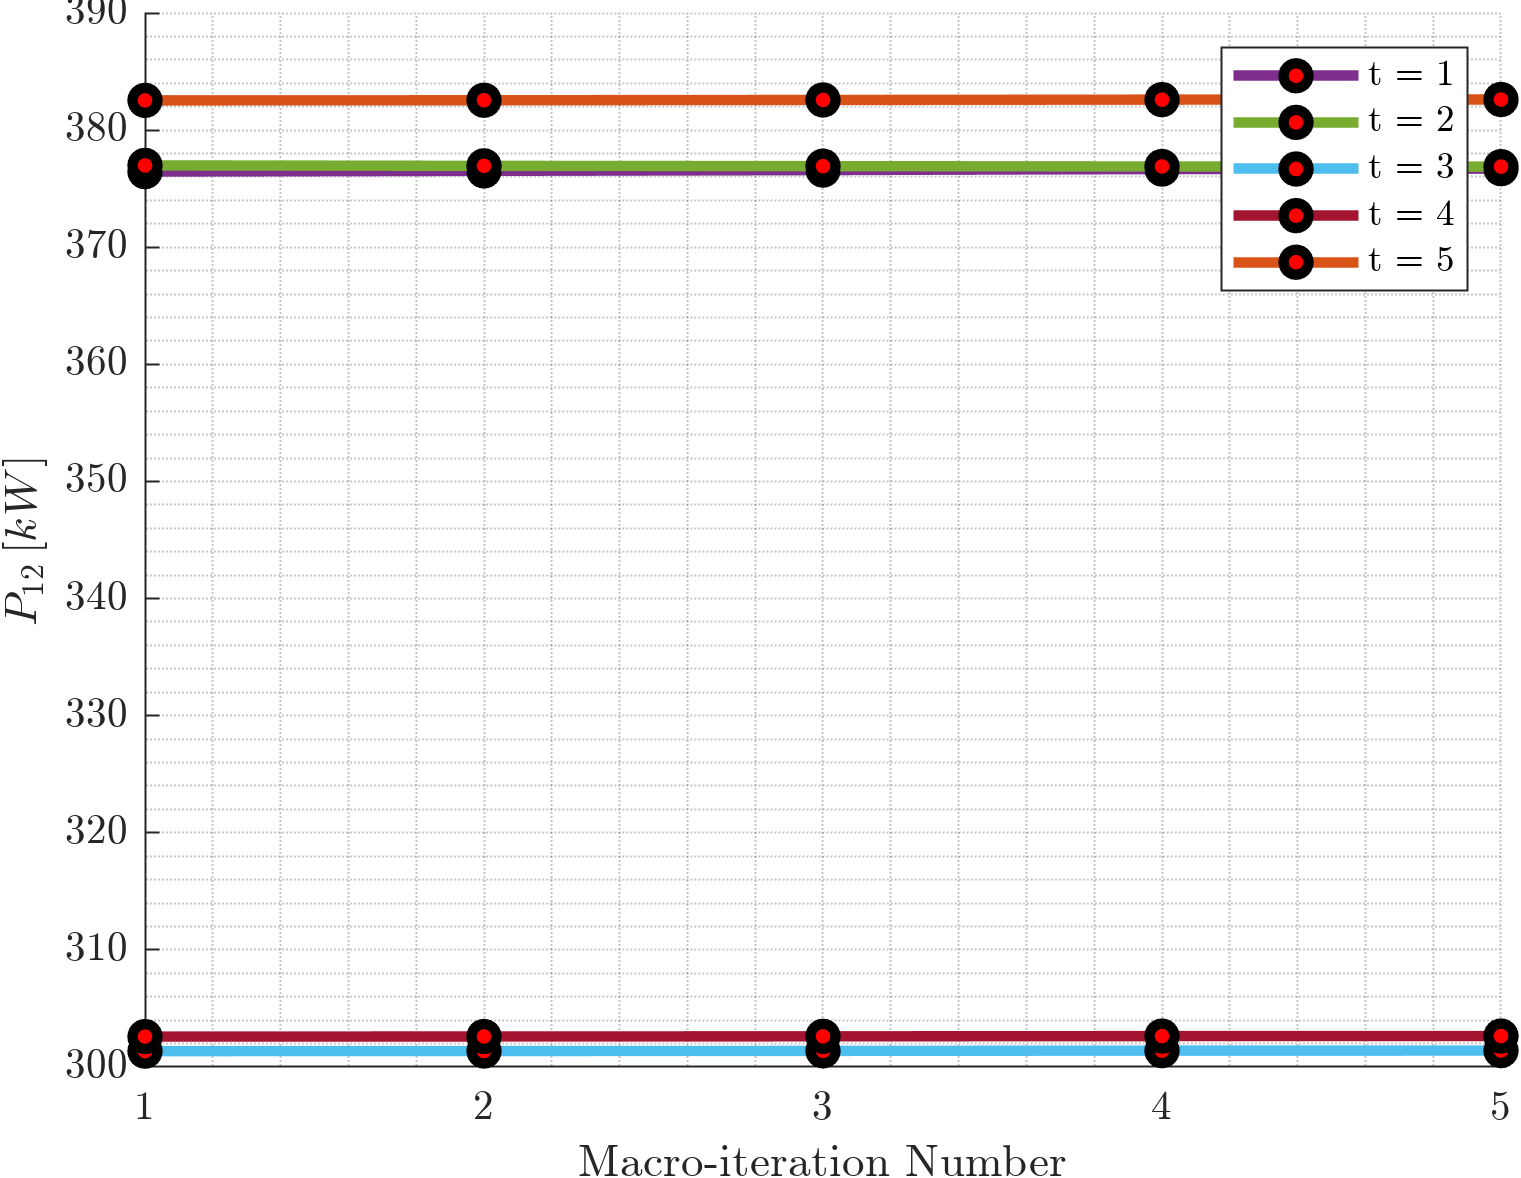
\includegraphics[width=\textwidth]{../figures/T5-pv20-batt30-genCost/dopf/convergenceCurves/BoundaryRealPower_vs_t_vs_macroItr_T_5_Areas_2_4_genCost_pv_20_batt_30_crop.png}
        \caption{\scriptsize Real Power flowing from Area $2$ into Area $4$}
        \label{fig:real_power_2_4}
    \end{subfigure}
    
    % Row 2
    \begin{subfigure}[b]{0.3\textwidth}
        \centering
        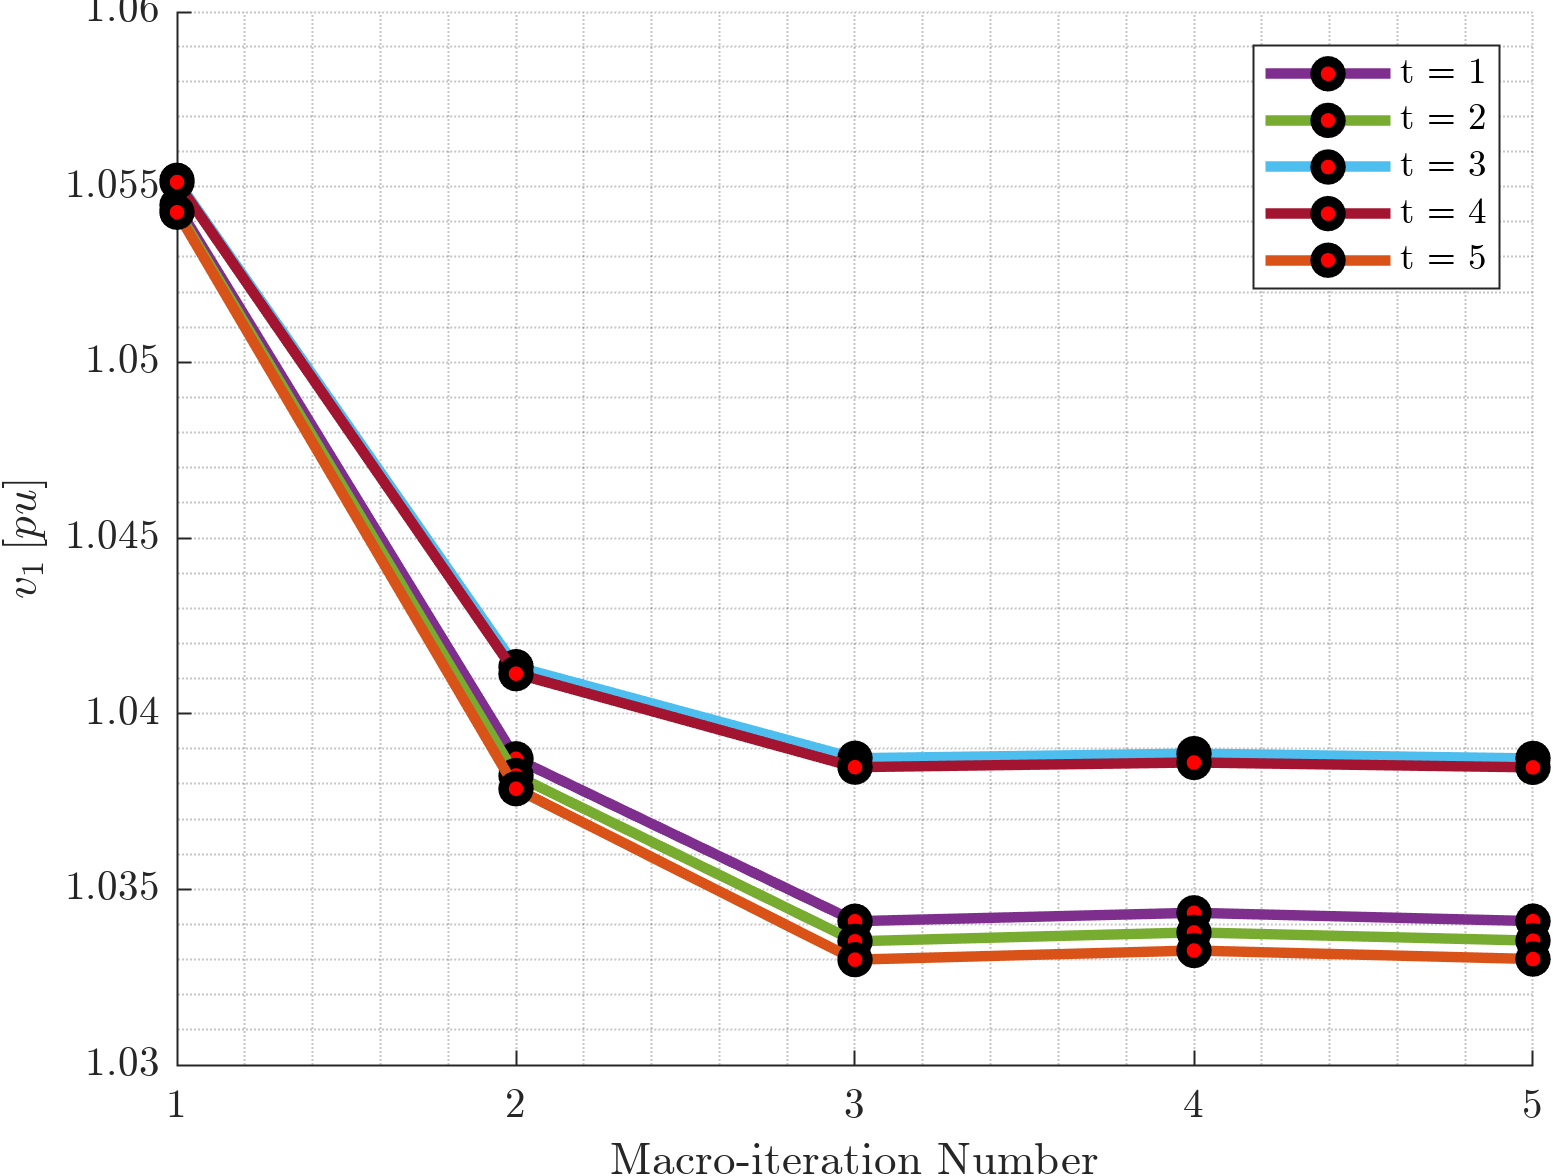
\includegraphics[width=\textwidth]{../figures/T5-pv20-batt30-genCost/dopf/convergenceCurves/BoundaryVoltage_vs_t_vs_macroItr_T_5_Areas_1_2_genCost_pv_20_batt_30_crop.png}
        \caption{\scriptsize Voltage at the PoI of Area $1$ and Area $2$}
        \label{fig:voltage_1_2}
    \end{subfigure}
    \hfill
    \begin{subfigure}[b]{0.3\textwidth}
        \centering
        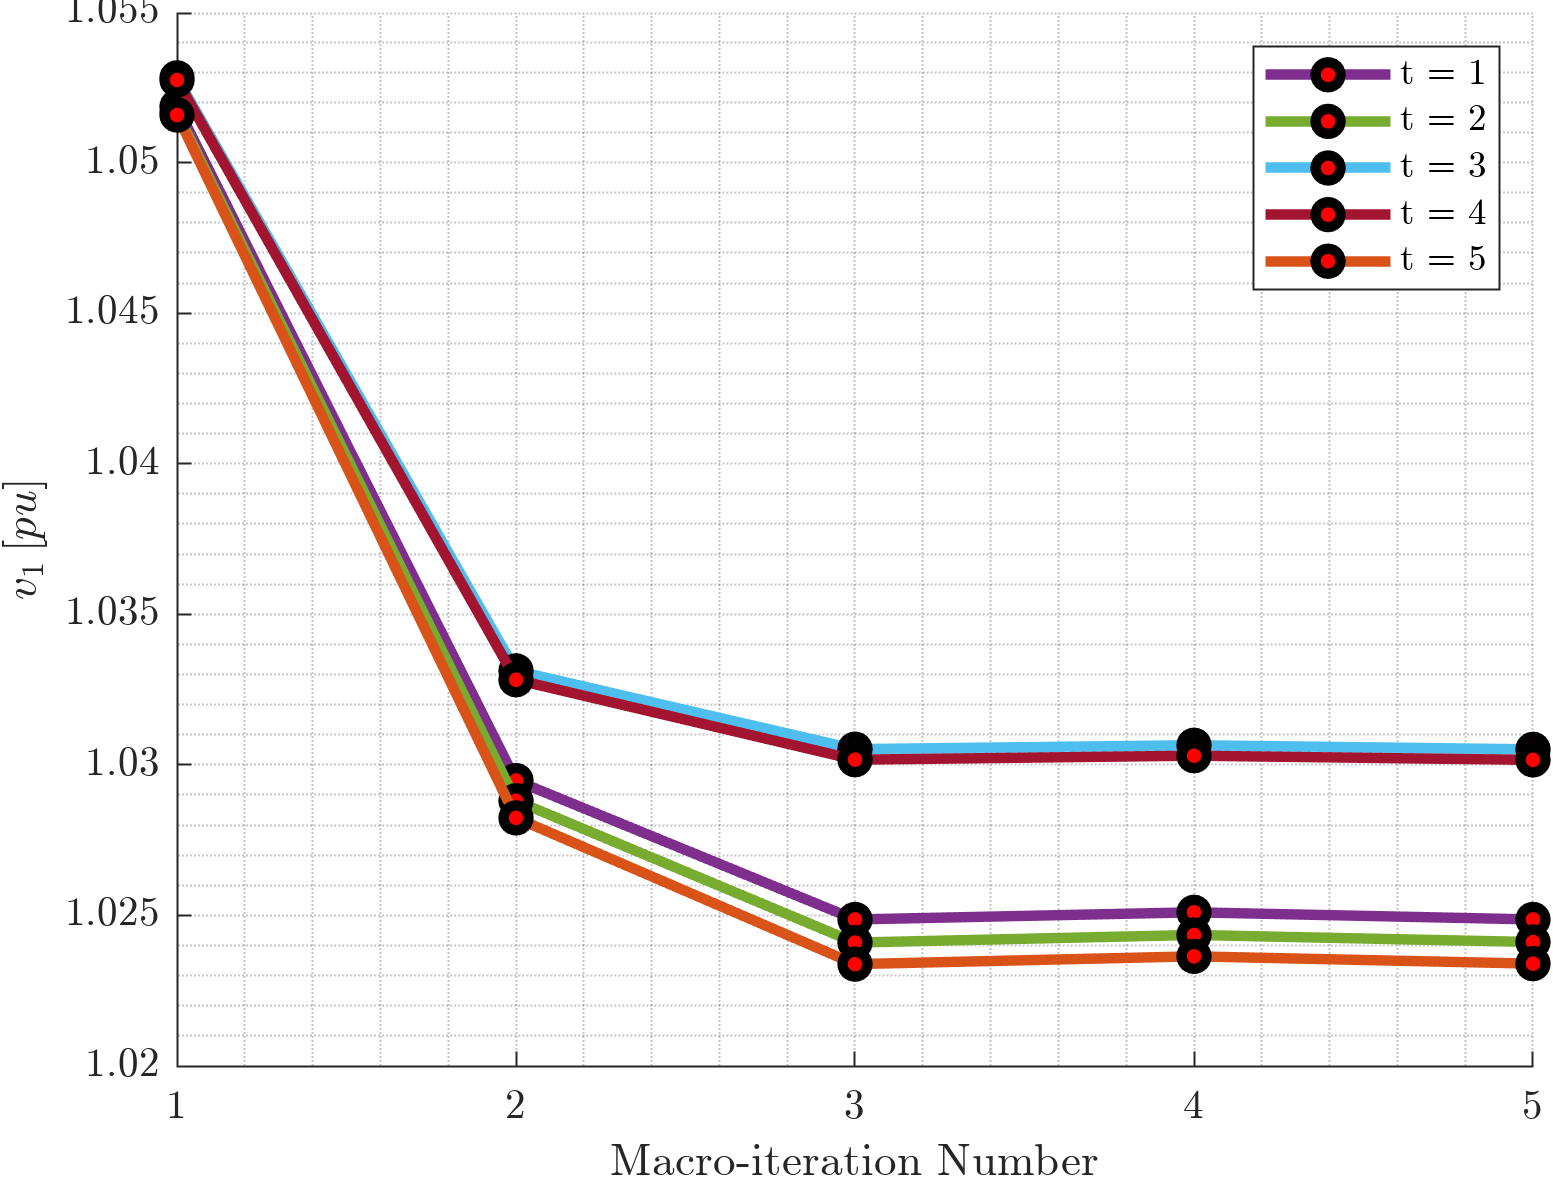
\includegraphics[width=\textwidth]{../figures/T5-pv20-batt30-genCost/dopf/convergenceCurves/BoundaryVoltage_vs_t_vs_macroItr_T_5_Areas_1_3_genCost_pv_20_batt_30_crop.png}
        \caption{\scriptsize Voltage at the PoI of Area $1$ and Area $3$}
        \label{fig:voltage_1_3}
    \end{subfigure}
    \hfill
    \begin{subfigure}[b]{0.3\textwidth}
        \centering
        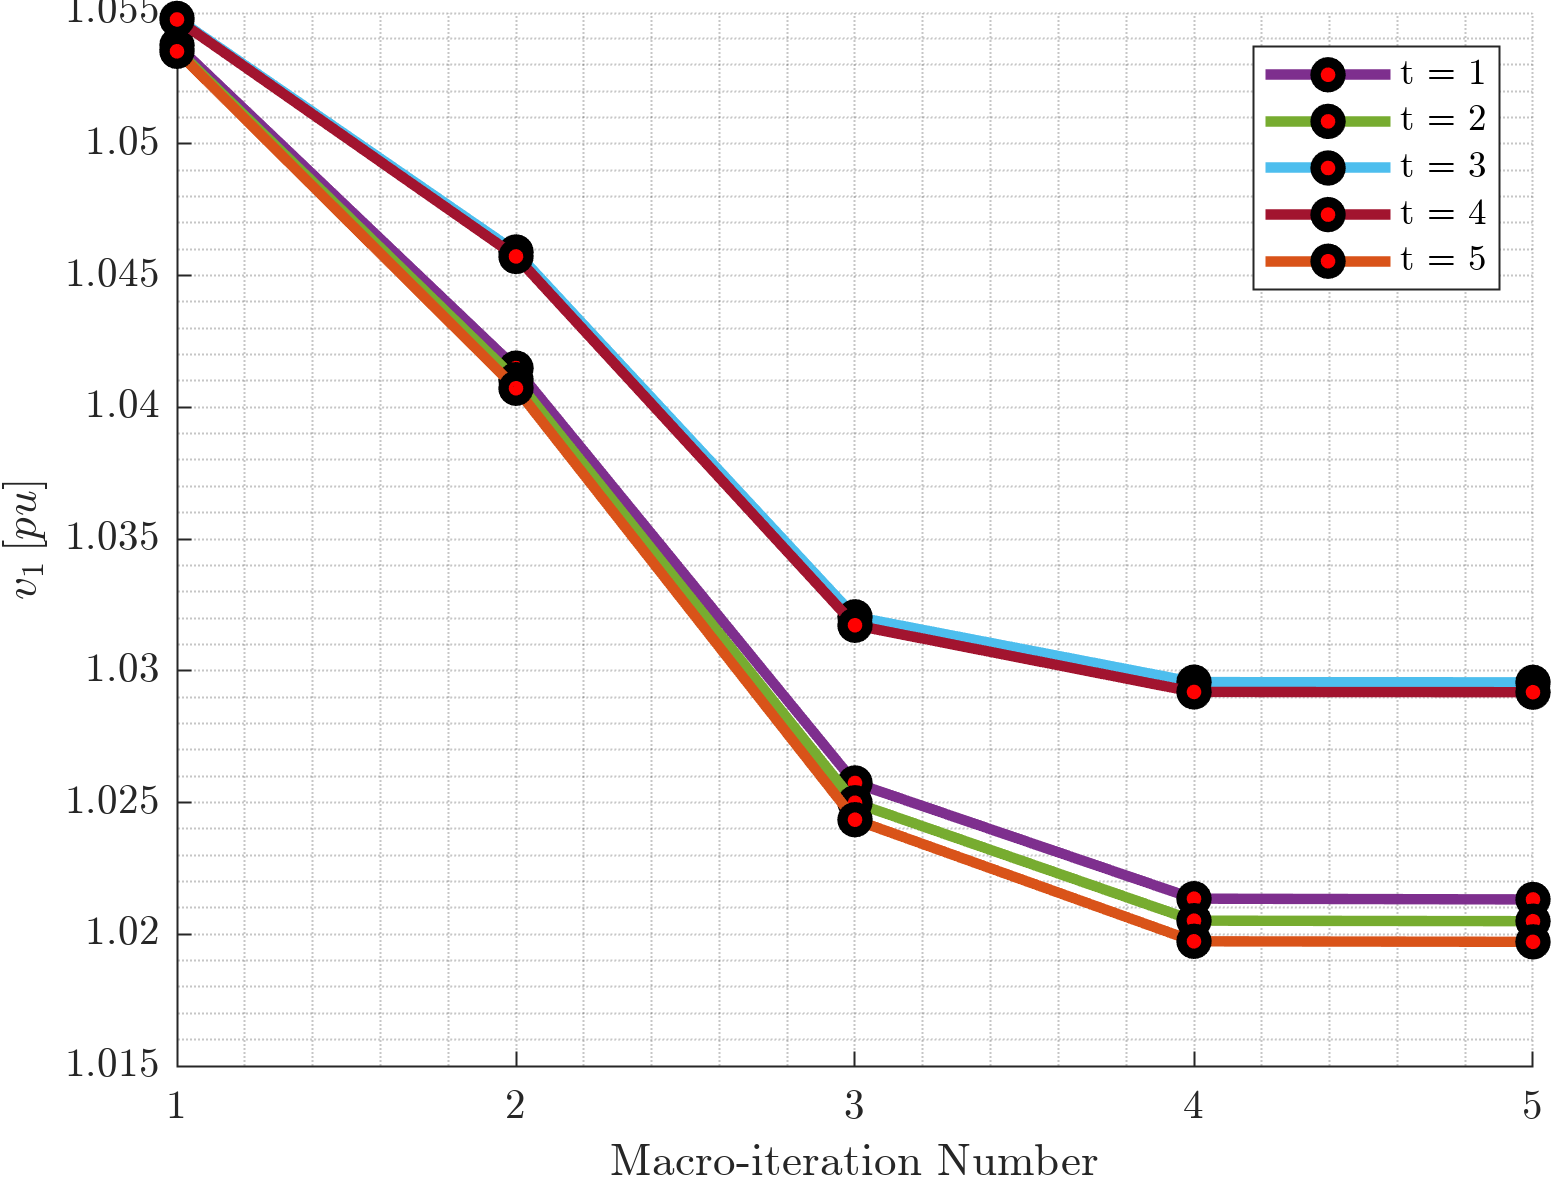
\includegraphics[width=\textwidth]{../figures/T5-pv20-batt30-genCost/dopf/convergenceCurves/BoundaryVoltage_vs_t_vs_macroItr_T_5_Areas_2_4_genCost_pv_20_batt_30_crop.png}
        \caption{\scriptsize Voltage at the PoI of Area $2$ and Area $4$}
        \label{fig:voltage_2_4}
    \end{subfigure}

    \caption{Convergence of Boundary variables with every iteration. Each plot represents a particular variable exchanged between a pair of connected areas. Each line graph within a plot represents a particular time period.}
    \label{fig:boundary_variables_all}
\end{figure*}

\begin{figure}[h!]
    \centering
    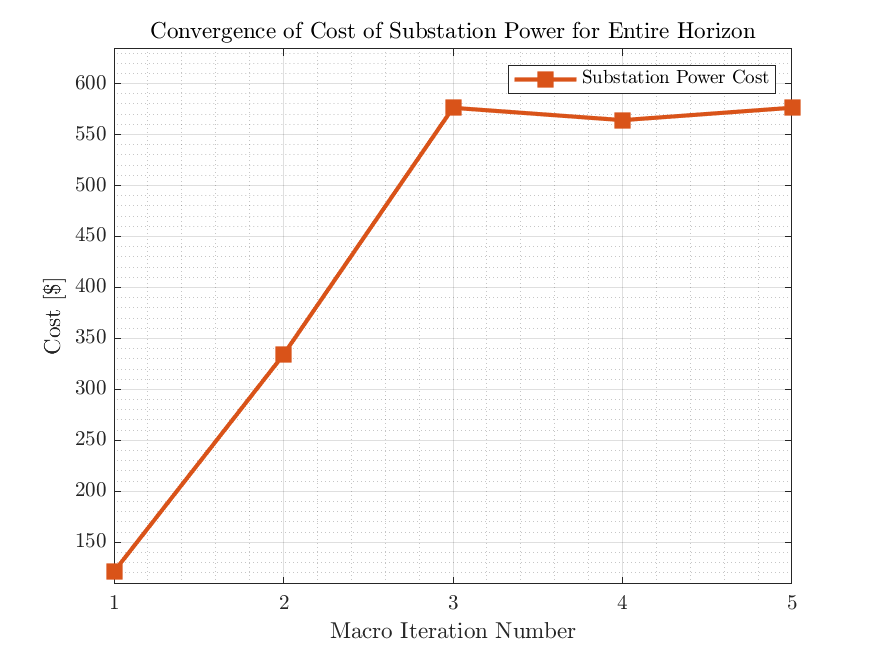
\includegraphics[height=0.25\textheight]{../figures/T5-pv20-batt30-genCost/dopf/outputCurves/ObjectiveConvergenceCurves_Horizon_5.png}
    \caption{Convergence of Objective Function Value with each MPDOPF iteration}
    \label{fig:outputConvergence-5-pv20-batt30-genCost}
\end{figure}

\subsection{Scalability Analysis}

To demonstrate the effectiveness of the proposed algorithm over a bigger horizon to demonstrate scalability, simulations were run for a $10$ time-period horizon. \Cref{fig:inputCurve-10} shows the forecasted profiles for load, solar irradiance and cost of substation power over the horizon. 

\subsubsection{Comparison between MPCOPF and MPDOPF}
In this section, comparative analyses are carried out between MPCOPF and MPDOPF considering 10-hour time steps with $20\%$ PV penetration and $30\%$ battery penetration.

\begin{figure}[h!]
    \centering
    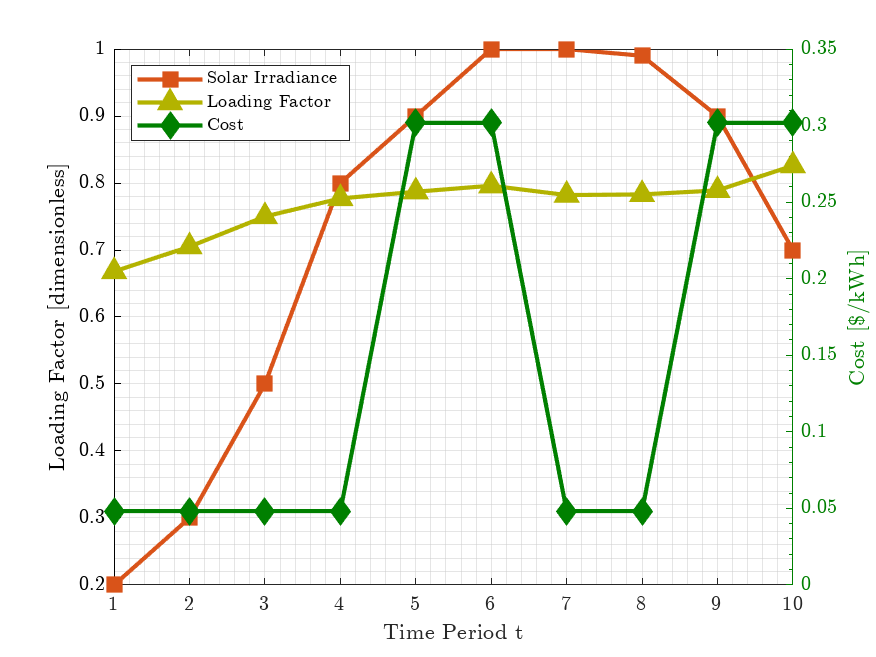
\includegraphics[height=0.25\textheight]{../figures/T10-inputCurves/InputCurves_Horizon_10.png}
    \caption{Forecasts for Demand Power, Irradiance and Cost of Substation Power over a 10 Hour Horizon}
    \label{fig:inputCurve-10}
\end{figure}

% \begin{table}[h!]
%     \centering
%     \caption{Comparative analyses between MPCOPF and MPDOPF - $10$ time-period horizon}
%     \begin{tabular}{|l|c|c|}
%     \hline
%     \textbf{Metric} & \textbf{MPCOPF} & \textbf{MPDOPF} \\ \hline
%     Substation power cost (\$) & 1197.87 & 1197.87 \\ \hline
%     Substation real power (kW) & 8544.28 & 8544.04 \\ \hline
%     Line loss (kW) & 148.67 & 148.94 \\ \hline
%     Substation reactive power (kVAR) & 1092.39 & 1252.03 \\ \hline
%     % PV real power (kW) & 561.26 & 561.26 \\ \hline
%     PV reactive power (kVAR) & 222.59 & 139.81 \\ \hline
%     Battery reactive power (kVAR) & 388.52 &  310.94 \\ \hline
%     Number of Iterations & - & 5 \\ \hline
%     Total Simulation Time (s) & 4620.73 & 358.69 \\ \hline
%     \end{tabular}
%     \label{table:opt-10-20-30}
% \end{table}

\begin{table}[h!]
    \centering
    \caption{Comparative analyses between MPCOPF and MPDOPF - $10$ time-period horizon}
    \begin{tabular}{|l|c|c|}
    \hline
    \textbf{Metric} & \textbf{MPCOPF} & \textbf{MPDOPF} \\ \hline
    Biggest subproblem size & \multicolumn{2}{c|}{} \\ \hline
    \quad Decision variables & {} & {} \\ \hline
    \quad Linear constraints & {} & {} \\ \hline
    \quad Nonlinear constraints & {} & {} \\ \hline
    Simulation results  & \multicolumn{2}{c|}{} \\ \hline
    \quad Substation power cost (\$) & 1197.87 & 1197.87 \\ \hline
    \quad Substation real power (kW) & 8544.28 & 8544.04 \\ \hline
    \quad Line loss (kW) & 148.67 & 148.94 \\ \hline
    \quad Substation reactive power (kVAR) & 1092.39 & 1252.03 \\ \hline
    \quad PV reactive power (kVAR) & 222.59 & 139.81 \\ \hline
    \quad Battery reactive power (kVAR) & 388.52 & 310.94 \\ \hline
    Computation  & \multicolumn{2}{c|}{} \\ \hline
    \quad Number of Iterations & - & 5 \\ \hline
    \quad Total Simulation Time (s) & 4620.73 & 358.69 \\ \hline
    \end{tabular}
    \label{table:opt-10-20-30}
\end{table}


Further, here the 

\begin{table}[h!]
    \centering
    \caption{ACOPF feasibility analyses - $10$ time-period horizon}
    \begin{tabular}{|l|c|c|}
    \hline
    \textbf{Metric} & \textbf{MPDOPF} & \textbf{OpenDSS} \\ \hline
    Full horizon  & \multicolumn{2}{c|}{} \\ \hline
    \quad Substation real power (kW) & 8544.04 & 8544.40 \\ \hline
    \quad Line loss (kW) & 148.94 & 148.87 \\ \hline
    \quad Substation reactive power (kVAR) & 1252.03 & 1243.36 \\ \hline
    Max. all-time discrepancy & \multicolumn{2}{c|}{} \\ \hline
    \quad Voltage (pu) & \multicolumn{2}{c|}{0.0002} \\ \hline
    \quad Line loss (kW) & \multicolumn{2}{c|}{0.0132} \\ \hline
    \quad Substation power (kW) & \multicolumn{2}{c|}{0.4002} \\ \hline
    \end{tabular}
    \label{table:feas-copf-10-20-30}
\end{table}

\begin{figure}[h!]
    \centering
    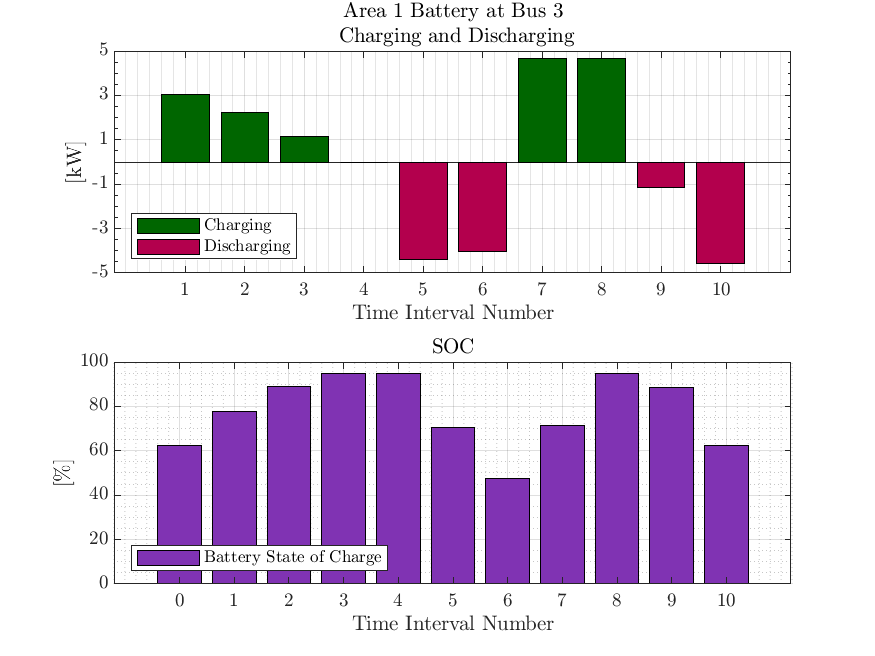
\includegraphics[width=\linewidth]{../figures/T10-pv20-batt30-genCost/dopf/BatteryPlots/macroItr_5_genCost_Battery_1_alpha_0.001.png}
    \caption{Charging-Discharging and SOC graphs for Battery at Bus 3 located in Area 1 obtained via MPDOPF}
    \label{fig:batt-plot-dopf-10-20-30-genCost}
\end{figure}
    

\lipsum[1]

\end{document}
